\documentclass[1p]{elsarticle_modified}
%\bibliographystyle{elsarticle-num}

%\usepackage[colorlinks]{hyperref}
%\usepackage{abbrmath_seonhwa} %\Abb, \Ascr, \Acal ,\Abf, \Afrak
\usepackage{amsfonts}
\usepackage{amssymb}
\usepackage{amsmath}
\usepackage{amsthm}
\usepackage{scalefnt}
\usepackage{amsbsy}
\usepackage{kotex}
\usepackage{caption}
\usepackage{subfig}
\usepackage{color}
\usepackage{graphicx}
\usepackage{xcolor} %% white, black, red, green, blue, cyan, magenta, yellow
\usepackage{float}
\usepackage{setspace}
\usepackage{hyperref}

\usepackage{tikz}
\usetikzlibrary{arrows}

\usepackage{multirow}
\usepackage{array} % fixed length table
\usepackage{hhline}

%%%%%%%%%%%%%%%%%%%%%
\makeatletter
\renewcommand*\env@matrix[1][\arraystretch]{%
	\edef\arraystretch{#1}%
	\hskip -\arraycolsep
	\let\@ifnextchar\new@ifnextchar
	\array{*\c@MaxMatrixCols c}}
\makeatother %https://tex.stackexchange.com/questions/14071/how-can-i-increase-the-line-spacing-in-a-matrix
%%%%%%%%%%%%%%%

\usepackage[normalem]{ulem}

\newcommand{\msout}[1]{\ifmmode\text{\sout{\ensuremath{#1}}}\else\sout{#1}\fi}
%SOURCE: \msout is \stkout macro in https://tex.stackexchange.com/questions/20609/strikeout-in-math-mode

\newcommand{\cancel}[1]{
	\ifmmode
	{\color{red}\msout{#1}}
	\else
	{\color{red}\sout{#1}}
	\fi
}

\newcommand{\add}[1]{
	{\color{blue}\uwave{#1}}
}

\newcommand{\replace}[2]{
	\ifmmode
	{\color{red}\msout{#1}}{\color{blue}\uwave{#2}}
	\else
	{\color{red}\sout{#1}}{\color{blue}\uwave{#2}}
	\fi
}

\newcommand{\Sol}{\mathcal{S}} %segment
\newcommand{\D}{D} %diagram
\newcommand{\A}{\mathcal{A}} %arc


%%%%%%%%%%%%%%%%%%%%%%%%%%%%%5 test

\def\sl{\operatorname{\textup{SL}}(2,\Cbb)}
\def\psl{\operatorname{\textup{PSL}}(2,\Cbb)}
\def\quan{\mkern 1mu \triangleright \mkern 1mu}

\theoremstyle{definition}
\newtheorem{thm}{Theorem}[section]
\newtheorem{prop}[thm]{Proposition}
\newtheorem{lem}[thm]{Lemma}
\newtheorem{ques}[thm]{Question}
\newtheorem{cor}[thm]{Corollary}
\newtheorem{defn}[thm]{Definition}
\newtheorem{exam}[thm]{Example}
\newtheorem{rmk}[thm]{Remark}
\newtheorem{alg}[thm]{Algorithm}

\newcommand{\I}{\sqrt{-1}}
\begin{document}

%\begin{frontmatter}
%
%\title{Boundary parabolic representations of knots up to 8 crossings}
%
%%% Group authors per affiliation:
%\author{Yunhi Cho} 
%\address{Department of Mathematics, University of Seoul, Seoul, Korea}
%\ead{yhcho@uos.ac.kr}
%
%
%\author{Seonhwa Kim} %\fnref{s_kim}}
%\address{Center for Geometry and Physics, Institute for Basic Science, Pohang, 37673, Korea}
%\ead{ryeona17@ibs.re.kr}
%
%\author{Hyuk Kim}
%\address{Department of Mathematical Sciences, Seoul National University, Seoul 08826, Korea}
%\ead{hyukkim@snu.ac.kr}
%
%\author{Seokbeom Yoon}
%\address{Department of Mathematical Sciences, Seoul National University, Seoul, 08826,  Korea}
%\ead{sbyoon15@snu.ac.kr}
%
%\begin{abstract}
%We find all boundary parabolic representation of knots up to 8 crossings.
%
%\end{abstract}
%\begin{keyword}
%    \MSC[2010] 57M25 
%\end{keyword}
%
%\end{frontmatter}

%\linenumbers
%\tableofcontents
%
\newcommand\colored[1]{\textcolor{white}{\rule[-0.35ex]{0.8em}{1.4ex}}\kern-0.8em\color{red} #1}%
%\newcommand\colored[1]{\textcolor{white}{ #1}\kern-2.17ex	\textcolor{white}{ #1}\kern-1.81ex	\textcolor{white}{ #1}\kern-2.15ex\color{red}#1	}

{\Large $\underline{12a_{0181}~(K12a_{0181})}$}

\setlength{\tabcolsep}{10pt}
\renewcommand{\arraystretch}{1.6}
\vspace{1cm}\begin{tabular}{m{100pt}>{\centering\arraybackslash}m{274pt}}
\multirow{5}{120pt}{
	\centering
	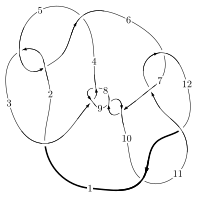
\includegraphics[width=112pt]{../../../GIT/diagram.site/Diagrams/png/982_12a_0181.png}\\
\ \ \ A knot diagram\footnotemark}&
\allowdisplaybreaks
\textbf{Linearized knot diagam} \\
\cline{2-2}
 &
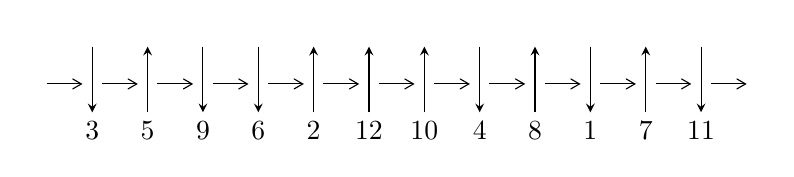
\begin{tikzpicture}[x=20pt, y=17pt]
	% nodes
	\node (C0) at (0, 0) {};
	\node (C1) at (1, 0) {};
	\node (C1U) at (1, +1) {};
	\node (C1D) at (1, -1) {3};

	\node (C2) at (2, 0) {};
	\node (C2U) at (2, +1) {};
	\node (C2D) at (2, -1) {5};

	\node (C3) at (3, 0) {};
	\node (C3U) at (3, +1) {};
	\node (C3D) at (3, -1) {9};

	\node (C4) at (4, 0) {};
	\node (C4U) at (4, +1) {};
	\node (C4D) at (4, -1) {6};

	\node (C5) at (5, 0) {};
	\node (C5U) at (5, +1) {};
	\node (C5D) at (5, -1) {2};

	\node (C6) at (6, 0) {};
	\node (C6U) at (6, +1) {};
	\node (C6D) at (6, -1) {12};

	\node (C7) at (7, 0) {};
	\node (C7U) at (7, +1) {};
	\node (C7D) at (7, -1) {10};

	\node (C8) at (8, 0) {};
	\node (C8U) at (8, +1) {};
	\node (C8D) at (8, -1) {4};

	\node (C9) at (9, 0) {};
	\node (C9U) at (9, +1) {};
	\node (C9D) at (9, -1) {8};

	\node (C10) at (10, 0) {};
	\node (C10U) at (10, +1) {};
	\node (C10D) at (10, -1) {1};

	\node (C11) at (11, 0) {};
	\node (C11U) at (11, +1) {};
	\node (C11D) at (11, -1) {7};

	\node (C12) at (12, 0) {};
	\node (C12U) at (12, +1) {};
	\node (C12D) at (12, -1) {11};
	\node (C13) at (13, 0) {};

	% arrows
	\draw[->,>={angle 60}]
	(C0) edge (C1) (C1) edge (C2) (C2) edge (C3) (C3) edge (C4) (C4) edge (C5) (C5) edge (C6) (C6) edge (C7) (C7) edge (C8) (C8) edge (C9) (C9) edge (C10) (C10) edge (C11) (C11) edge (C12) (C12) edge (C13) ;	\draw[->,>=stealth]
	(C1U) edge (C1D) (C2D) edge (C2U) (C3U) edge (C3D) (C4U) edge (C4D) (C5D) edge (C5U) (C6D) edge (C6U) (C7D) edge (C7U) (C8U) edge (C8D) (C9D) edge (C9U) (C10U) edge (C10D) (C11D) edge (C11U) (C12U) edge (C12D) ;
	\end{tikzpicture} \\
\hhline{~~} \\& 
\textbf{Solving Sequence} \\ \cline{2-2} 
 &
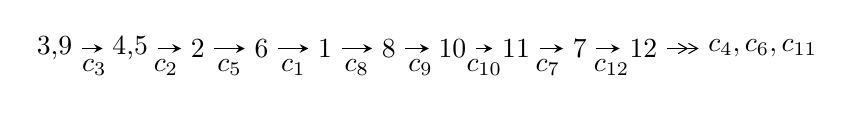
\begin{tikzpicture}[x=23pt, y=7pt]
	% node
	\node (A0) at (-1/8, 0) {3,9};
	\node (A1) at (17/16, 0) {4,5};
	\node (A2) at (17/8, 0) {2};
	\node (A3) at (25/8, 0) {6};
	\node (A4) at (33/8, 0) {1};
	\node (A5) at (41/8, 0) {8};
	\node (A6) at (49/8, 0) {10};
	\node (A7) at (57/8, 0) {11};
	\node (A8) at (65/8, 0) {7};
	\node (A9) at (73/8, 0) {12};
	\node (C1) at (1/2, -1) {$c_{3}$};
	\node (C2) at (13/8, -1) {$c_{2}$};
	\node (C3) at (21/8, -1) {$c_{5}$};
	\node (C4) at (29/8, -1) {$c_{1}$};
	\node (C5) at (37/8, -1) {$c_{8}$};
	\node (C6) at (45/8, -1) {$c_{9}$};
	\node (C7) at (53/8, -1) {$c_{10}$};
	\node (C8) at (61/8, -1) {$c_{7}$};
	\node (C9) at (69/8, -1) {$c_{12}$};
	\node (A10) at (11, 0) {$c_{4},c_{6},c_{11}$};

	% edge
	\draw[->,>=stealth]	
	(A0) edge (A1) (A1) edge (A2) (A2) edge (A3) (A3) edge (A4) (A4) edge (A5) (A5) edge (A6) (A6) edge (A7) (A7) edge (A8) (A8) edge (A9) ;
	\draw[->>,>={angle 60}]	
	(A9) edge (A10);
\end{tikzpicture} \\ 

\end{tabular} \\

\footnotetext{
The image of knot diagram is generated by the software ``\textbf{Draw programme}" developed by Andrew Bartholomew(\url{http://www.layer8.co.uk/maths/draw/index.htm\#Running-draw}), where we modified some parts for our purpose(\url{https://github.com/CATsTAILs/LinksPainter}).
}\phantom \\ \newline 
\centering \textbf{Ideals for irreducible components\footnotemark of $X_{\text{par}}$} 
 
\begin{align*}
I^u_{1}&=\langle 
u^{19}+3 u^{18}+\cdots+4 b+2 u,\;- u^{18}-3 u^{17}+\cdots+4 a-6,\;u^{20}+5 u^{19}+\cdots+12 u+4\rangle \\
I^u_{2}&=\langle 
-82 u^{32} a+53 u^{32}+\cdots+116 a+32,\;2 u^{32} a+u^{32}+\cdots+12 a-17,\;u^{33}-2 u^{32}+\cdots- u+2\rangle \\
\\
I^v_{1}&=\langle 
a,\;b^2+b+1,\;v+1\rangle \\
I^v_{2}&=\langle 
a,\;b- v+1,\;v^2- v+1\rangle \\
\end{align*}
\raggedright * 4 irreducible components of $\dim_{\mathbb{C}}=0$, with total 90 representations.\\
\footnotetext{All coefficients of polynomials are rational numbers. But the coefficients are sometimes approximated in decimal forms when there is not enough margin.}
\newpage
\renewcommand{\arraystretch}{1}
\centering \section*{I. $I^u_{1}= \langle u^{19}+3 u^{18}+\cdots+4 b+2 u,\;- u^{18}-3 u^{17}+\cdots+4 a-6,\;u^{20}+5 u^{19}+\cdots+12 u+4 \rangle$}
\flushleft \textbf{(i) Arc colorings}\\
\begin{tabular}{m{7pt} m{180pt} m{7pt} m{180pt} }
\flushright $a_{3}=$&$\begin{pmatrix}1\\0\end{pmatrix}$ \\
\flushright $a_{9}=$&$\begin{pmatrix}0\\u\end{pmatrix}$ \\
\flushright $a_{4}=$&$\begin{pmatrix}1\\u^2\end{pmatrix}$ \\
\flushright $a_{5}=$&$\begin{pmatrix}\frac{1}{4} u^{18}+\frac{3}{4} u^{17}+\cdots+u+\frac{3}{2}\\-\frac{1}{4} u^{19}-\frac{3}{4} u^{18}+\cdots-\frac{9}{4} u^3-\frac{1}{2} u\end{pmatrix}$ \\
\flushright $a_{2}=$&$\begin{pmatrix}-\frac{7}{4} u^{19}-8 u^{18}+\cdots-15 u-\frac{9}{2}\\-\frac{3}{4} u^{19}-\frac{15}{4} u^{18}+\cdots-\frac{19}{2} u-4\end{pmatrix}$ \\
\flushright $a_{6}=$&$\begin{pmatrix}-\frac{7}{4} u^{19}-8 u^{18}+\cdots-15 u-\frac{9}{2}\\\frac{9}{4} u^{19}+\frac{31}{4} u^{18}+\cdots+\frac{15}{2} u+1\end{pmatrix}$ \\
\flushright $a_{1}=$&$\begin{pmatrix}-\frac{5}{2} u^{19}-\frac{47}{4} u^{18}+\cdots-\frac{49}{2} u-\frac{17}{2}\\-\frac{3}{4} u^{19}-\frac{15}{4} u^{18}+\cdots-\frac{19}{2} u-4\end{pmatrix}$ \\
\flushright $a_{8}=$&$\begin{pmatrix}u\\u^3+u\end{pmatrix}$ \\
\flushright $a_{10}=$&$\begin{pmatrix}u^3\\u^5+u^3+u\end{pmatrix}$ \\
\flushright $a_{11}=$&$\begin{pmatrix}-\frac{1}{4} u^{19}- u^{18}+\cdots-\frac{3}{2} u-\frac{1}{2}\\-\frac{1}{4} u^{19}-\frac{5}{4} u^{18}+\cdots-\frac{3}{2} u-1\end{pmatrix}$ \\
\flushright $a_{7}=$&$\begin{pmatrix}u^5+u\\u^7+u^5+2 u^3+u\end{pmatrix}$ \\
\flushright $a_{12}=$&$\begin{pmatrix}-\frac{7}{4} u^{19}-7 u^{18}+\cdots-\frac{21}{2} u-\frac{7}{2}\\-\frac{7}{4} u^{19}-\frac{37}{4} u^{18}+\cdots-\frac{37}{2} u-8\end{pmatrix}$\\&\end{tabular}
\flushleft \textbf{(ii) Obstruction class $= -1$}\\~\\
\flushleft \textbf{(iii) Cusp Shapes $= -13 u^{19}-66 u^{18}-180 u^{17}-337 u^{16}-477 u^{15}-527 u^{14}-374 u^{13}-30 u^{12}+397 u^{11}+641 u^{10}+698 u^9+494 u^8+210 u^7-106 u^6-168 u^5-196 u^4-209 u^3-259 u^2-158 u-62$}\\~\\
\newpage\renewcommand{\arraystretch}{1}
\flushleft \textbf{(iv) u-Polynomials at the component}\newline \\
\begin{tabular}{m{50pt}|m{274pt}}
Crossings & \hspace{64pt}u-Polynomials at each crossing \\
\hline $$\begin{aligned}c_{1},c_{4},c_{10}\\c_{12}\end{aligned}$$&$\begin{aligned}
&u^{20}+7 u^{19}+\cdots+6 u+1
\end{aligned}$\\
\hline $$\begin{aligned}c_{2},c_{5},c_{6}\\c_{11}\end{aligned}$$&$\begin{aligned}
&u^{20}+u^{19}+\cdots-2 u+1
\end{aligned}$\\
\hline $$\begin{aligned}c_{3},c_{8}\end{aligned}$$&$\begin{aligned}
&u^{20}+5 u^{19}+\cdots+12 u+4
\end{aligned}$\\
\hline $$\begin{aligned}c_{7},c_{9}\end{aligned}$$&$\begin{aligned}
&u^{20}-5 u^{19}+\cdots-48 u+16
\end{aligned}$\\
\hline
\end{tabular}\\~\\
\newpage\renewcommand{\arraystretch}{1}
\flushleft \textbf{(v) Riley Polynomials at the component}\newline \\
\begin{tabular}{m{50pt}|m{274pt}}
Crossings & \hspace{64pt}Riley Polynomials at each crossing \\
\hline $$\begin{aligned}c_{1},c_{4},c_{10}\\c_{12}\end{aligned}$$&$\begin{aligned}
&y^{20}+15 y^{19}+\cdots+42 y+1
\end{aligned}$\\
\hline $$\begin{aligned}c_{2},c_{5},c_{6}\\c_{11}\end{aligned}$$&$\begin{aligned}
&y^{20}+7 y^{19}+\cdots+6 y+1
\end{aligned}$\\
\hline $$\begin{aligned}c_{3},c_{8}\end{aligned}$$&$\begin{aligned}
&y^{20}+5 y^{19}+\cdots+48 y+16
\end{aligned}$\\
\hline $$\begin{aligned}c_{7},c_{9}\end{aligned}$$&$\begin{aligned}
&y^{20}+13 y^{19}+\cdots+2560 y+256
\end{aligned}$\\
\hline
\end{tabular}\\~\\
\newpage\flushleft \textbf{(vi) Complex Volumes and Cusp Shapes}
$$\begin{array}{c|c|c}  
\text{Solutions to }I^u_{1}& \I (\text{vol} + \sqrt{-1}CS) & \text{Cusp shape}\\
 \hline 
\begin{aligned}
u &= \phantom{-}0.956413 + 0.106188 I \\
a &= \phantom{-}0.666389 - 0.362681 I \\
b &= -0.690206 - 0.870989 I\end{aligned}
 & \phantom{-}3.29641 + 5.31416 I & \phantom{-}3.14759 - 6.32881 I \\ \hline\begin{aligned}
u &= \phantom{-}0.956413 - 0.106188 I \\
a &= \phantom{-}0.666389 + 0.362681 I \\
b &= -0.690206 + 0.870989 I\end{aligned}
 & \phantom{-}3.29641 - 5.31416 I & \phantom{-}3.14759 + 6.32881 I \\ \hline\begin{aligned}
u &= -0.859253 + 0.598044 I \\
a &= \phantom{-}0.726799 - 0.250535 I \\
b &= -0.710902 - 0.608435 I\end{aligned}
 & \phantom{-}0.831191 + 0.623147 I & \phantom{-}2.59573 - 2.24523 I \\ \hline\begin{aligned}
u &= -0.859253 - 0.598044 I \\
a &= \phantom{-}0.726799 + 0.250535 I \\
b &= -0.710902 + 0.608435 I\end{aligned}
 & \phantom{-}0.831191 - 0.623147 I & \phantom{-}2.59573 + 2.24523 I \\ \hline\begin{aligned}
u &= \phantom{-}0.511571 + 0.639622 I \\
a &= \phantom{-}1.075070 + 0.676318 I \\
b &= -0.102085 + 0.859228 I\end{aligned}
 & -2.97361 - 1.87280 I & -8.34696 + 4.79097 I \\ \hline\begin{aligned}
u &= \phantom{-}0.511571 - 0.639622 I \\
a &= \phantom{-}1.075070 - 0.676318 I \\
b &= -0.102085 - 0.859228 I\end{aligned}
 & -2.97361 + 1.87280 I & -8.34696 - 4.79097 I \\ \hline\begin{aligned}
u &= \phantom{-}0.193921 + 1.176600 I \\
a &= -1.33172 - 1.10006 I \\
b &= \phantom{-}0.775256 + 0.795478 I\end{aligned}
 & \phantom{-}8.04637 + 1.61009 I & \phantom{-}7.70402 - 2.24180 I \\ \hline\begin{aligned}
u &= \phantom{-}0.193921 - 1.176600 I \\
a &= -1.33172 + 1.10006 I \\
b &= \phantom{-}0.775256 - 0.795478 I\end{aligned}
 & \phantom{-}8.04637 - 1.61009 I & \phantom{-}7.70402 + 2.24180 I \\ \hline\begin{aligned}
u &= -0.962446 + 0.718212 I \\
a &= \phantom{-}0.613669 + 0.425585 I \\
b &= -0.666520 + 1.031640 I\end{aligned}
 & -1.66717 - 10.06630 I & -1.36976 + 7.52063 I \\ \hline\begin{aligned}
u &= -0.962446 - 0.718212 I \\
a &= \phantom{-}0.613669 - 0.425585 I \\
b &= -0.666520 - 1.031640 I\end{aligned}
 & -1.66717 + 10.06630 I & -1.36976 - 7.52063 I\\
 \hline 
 \end{array}$$\newpage$$\begin{array}{c|c|c}  
\text{Solutions to }I^u_{1}& \I (\text{vol} + \sqrt{-1}CS) & \text{Cusp shape}\\
 \hline 
\begin{aligned}
u &= -0.824880 + 0.894608 I \\
a &= \phantom{-}0.753015 - 1.021300 I \\
b &= -0.023434 - 1.120850 I\end{aligned}
 & -9.84057 + 3.07245 I & -9.39268 - 2.83211 I \\ \hline\begin{aligned}
u &= -0.824880 - 0.894608 I \\
a &= \phantom{-}0.753015 + 1.021300 I \\
b &= -0.023434 + 1.120850 I\end{aligned}
 & -9.84057 - 3.07245 I & -9.39268 + 2.83211 I \\ \hline\begin{aligned}
u &= \phantom{-}0.337755 + 1.176280 I \\
a &= -2.12989 + 0.17473 I \\
b &= \phantom{-}0.738480 - 0.944822 I\end{aligned}
 & \phantom{-}7.12649 - 9.83704 I & \phantom{-}5.40465 + 9.06026 I \\ \hline\begin{aligned}
u &= \phantom{-}0.337755 - 1.176280 I \\
a &= -2.12989 - 0.17473 I \\
b &= \phantom{-}0.738480 + 0.944822 I\end{aligned}
 & \phantom{-}7.12649 + 9.83704 I & \phantom{-}5.40465 - 9.06026 I \\ \hline\begin{aligned}
u &= -0.716852 + 1.049790 I \\
a &= -0.357717 + 0.974184 I \\
b &= \phantom{-}0.809192 - 0.602967 I\end{aligned}
 & \phantom{-}2.16361 + 5.20834 I & \phantom{-}3.98742 - 2.19274 I \\ \hline\begin{aligned}
u &= -0.716852 - 1.049790 I \\
a &= -0.357717 - 0.974184 I \\
b &= \phantom{-}0.809192 + 0.602967 I\end{aligned}
 & \phantom{-}2.16361 - 5.20834 I & \phantom{-}3.98742 + 2.19274 I \\ \hline\begin{aligned}
u &= -0.342141 + 0.579550 I \\
a &= \phantom{-}0.950288 - 0.152216 I \\
b &= -0.318780 - 0.354384 I\end{aligned}
 & \phantom{-}0.155657 + 1.086730 I & \phantom{-}2.50050 - 5.83378 I \\ \hline\begin{aligned}
u &= -0.342141 - 0.579550 I \\
a &= \phantom{-}0.950288 + 0.152216 I \\
b &= -0.318780 + 0.354384 I\end{aligned}
 & \phantom{-}0.155657 - 1.086730 I & \phantom{-}2.50050 + 5.83378 I \\ \hline\begin{aligned}
u &= -0.794089 + 1.065150 I \\
a &= -1.96591 + 0.82985 I \\
b &= \phantom{-}0.688998 + 1.054600 I\end{aligned}
 & -0.5586 + 16.5027 I & -0.23050 - 11.16239 I \\ \hline\begin{aligned}
u &= -0.794089 - 1.065150 I \\
a &= -1.96591 - 0.82985 I \\
b &= \phantom{-}0.688998 - 1.054600 I\end{aligned}
 & -0.5586 - 16.5027 I & -0.23050 + 11.16239 I\\
 \hline 
 \end{array}$$\newpage\newpage\renewcommand{\arraystretch}{1}
\centering \section*{II. $I^u_{2}= \langle -82 u^{32} a+53 u^{32}+\cdots+116 a+32,\;2 u^{32} a+u^{32}+\cdots+12 a-17,\;u^{33}-2 u^{32}+\cdots- u+2 \rangle$}
\flushleft \textbf{(i) Arc colorings}\\
\begin{tabular}{m{7pt} m{180pt} m{7pt} m{180pt} }
\flushright $a_{3}=$&$\begin{pmatrix}1\\0\end{pmatrix}$ \\
\flushright $a_{9}=$&$\begin{pmatrix}0\\u\end{pmatrix}$ \\
\flushright $a_{4}=$&$\begin{pmatrix}1\\u^2\end{pmatrix}$ \\
\flushright $a_{5}=$&$\begin{pmatrix}a\\1.20588 a u^{32}-0.779412 u^{32}+\cdots-1.70588 a-0.470588\end{pmatrix}$ \\
\flushright $a_{2}=$&$\begin{pmatrix}1.27941 a u^{32}-0.147059 u^{32}+\cdots+0.470588 a-1.60294\\0.514706 a u^{32}+0.426471 u^{32}+\cdots-1.26471 a-0.176471\end{pmatrix}$ \\
\flushright $a_{6}=$&$\begin{pmatrix}1.27941 a u^{32}-0.147059 u^{32}+\cdots+0.470588 a-1.60294\\-0.647059 a u^{32}-1.26471 u^{32}+\cdots-1.35294 a+2.26471\end{pmatrix}$ \\
\flushright $a_{1}=$&$\begin{pmatrix}1.79412 a u^{32}+0.279412 u^{32}+\cdots-0.794118 a-1.77941\\0.514706 a u^{32}+0.426471 u^{32}+\cdots-1.26471 a-0.176471\end{pmatrix}$ \\
\flushright $a_{8}=$&$\begin{pmatrix}u\\u^3+u\end{pmatrix}$ \\
\flushright $a_{10}=$&$\begin{pmatrix}u^3\\u^5+u^3+u\end{pmatrix}$ \\
\flushright $a_{11}=$&$\begin{pmatrix}-0.911765 a u^{32}+1.05882 u^{32}+\cdots+2.91176 a-1.30882\\- u^{32}+2 u^{31}+\cdots-\frac{1}{2} u+2\end{pmatrix}$ \\
\flushright $a_{7}=$&$\begin{pmatrix}u^5+u\\u^7+u^5+2 u^3+u\end{pmatrix}$ \\
\flushright $a_{12}=$&$\begin{pmatrix}-0.911765 a u^{32}+1.55882 u^{32}+\cdots+2.91176 a-0.308824\\1.35294 a u^{32}-1.01471 u^{32}+\cdots-1.35294 a+1.26471\end{pmatrix}$\\&\end{tabular}
\flushleft \textbf{(ii) Obstruction class $= -1$}\\~\\
\flushleft \textbf{(iii) Cusp Shapes $= - u^{32}-2 u^{31}-3 u^{30}-8 u^{29}-11 u^{28}-28 u^{27}-26 u^{26}-60 u^{25}-55 u^{24}-114 u^{23}-106 u^{22}-160 u^{21}-162 u^{20}-198 u^{19}-234 u^{18}-196 u^{17}-257 u^{16}-162 u^{15}-244 u^{14}-124 u^{13}-166 u^{12}-72 u^{11}-64 u^{10}-54 u^9+4 u^8-28 u^7+34 u^6-16 u^5+22 u^4-6 u^3+4 u^2-2 u+1$}\\~\\
\newpage\renewcommand{\arraystretch}{1}
\flushleft \textbf{(iv) u-Polynomials at the component}\newline \\
\begin{tabular}{m{50pt}|m{274pt}}
Crossings & \hspace{64pt}u-Polynomials at each crossing \\
\hline $$\begin{aligned}c_{1},c_{4},c_{10}\\c_{12}\end{aligned}$$&$\begin{aligned}
&u^{66}+24 u^{65}+\cdots+17 u+1
\end{aligned}$\\
\hline $$\begin{aligned}c_{2},c_{5},c_{6}\\c_{11}\end{aligned}$$&$\begin{aligned}
&u^{66}+2 u^{65}+\cdots+u+1
\end{aligned}$\\
\hline $$\begin{aligned}c_{3},c_{8}\end{aligned}$$&$\begin{aligned}
&(u^{33}-2 u^{32}+\cdots- u+2)^{2}
\end{aligned}$\\
\hline $$\begin{aligned}c_{7},c_{9}\end{aligned}$$&$\begin{aligned}
&(u^{33}-10 u^{32}+\cdots-23 u+4)^{2}
\end{aligned}$\\
\hline
\end{tabular}\\~\\
\newpage\renewcommand{\arraystretch}{1}
\flushleft \textbf{(v) Riley Polynomials at the component}\newline \\
\begin{tabular}{m{50pt}|m{274pt}}
Crossings & \hspace{64pt}Riley Polynomials at each crossing \\
\hline $$\begin{aligned}c_{1},c_{4},c_{10}\\c_{12}\end{aligned}$$&$\begin{aligned}
&y^{66}+36 y^{65}+\cdots+97 y+1
\end{aligned}$\\
\hline $$\begin{aligned}c_{2},c_{5},c_{6}\\c_{11}\end{aligned}$$&$\begin{aligned}
&y^{66}+24 y^{65}+\cdots+17 y+1
\end{aligned}$\\
\hline $$\begin{aligned}c_{3},c_{8}\end{aligned}$$&$\begin{aligned}
&(y^{33}+10 y^{32}+\cdots-23 y-4)^{2}
\end{aligned}$\\
\hline $$\begin{aligned}c_{7},c_{9}\end{aligned}$$&$\begin{aligned}
&(y^{33}+26 y^{32}+\cdots-335 y-16)^{2}
\end{aligned}$\\
\hline
\end{tabular}\\~\\
\newpage\flushleft \textbf{(vi) Complex Volumes and Cusp Shapes}
$$\begin{array}{c|c|c}  
\text{Solutions to }I^u_{2}& \I (\text{vol} + \sqrt{-1}CS) & \text{Cusp shape}\\
 \hline 
\begin{aligned}
u &= -0.049702 + 0.985538 I \\
a &= \phantom{-}0.804899 - 0.013377 I \\
b &= -0.628084 - 0.033140 I\end{aligned}
 & \phantom{-}4.01597 + 2.68651 I & \phantom{-}7.73425 - 3.44417 I \\ \hline\begin{aligned}
u &= -0.049702 + 0.985538 I \\
a &= -2.27679 - 1.25073 I \\
b &= \phantom{-}0.701064 + 0.855945 I\end{aligned}
 & \phantom{-}4.01597 + 2.68651 I & \phantom{-}7.73425 - 3.44417 I \\ \hline\begin{aligned}
u &= -0.049702 - 0.985538 I \\
a &= \phantom{-}0.804899 + 0.013377 I \\
b &= -0.628084 + 0.033140 I\end{aligned}
 & \phantom{-}4.01597 - 2.68651 I & \phantom{-}7.73425 + 3.44417 I \\ \hline\begin{aligned}
u &= -0.049702 - 0.985538 I \\
a &= -2.27679 + 1.25073 I \\
b &= \phantom{-}0.701064 - 0.855945 I\end{aligned}
 & \phantom{-}4.01597 - 2.68651 I & \phantom{-}7.73425 + 3.44417 I \\ \hline\begin{aligned}
u &= \phantom{-}0.665379 + 0.776145 I \\
a &= \phantom{-}0.635938 - 0.460788 I \\
b &= -0.589255 - 1.034860 I\end{aligned}
 & -0.77598 + 2.47863 I & \phantom{-}0.24297 - 1.77615 I \\ \hline\begin{aligned}
u &= \phantom{-}0.665379 + 0.776145 I \\
a &= \phantom{-}0.110839 - 1.231880 I \\
b &= \phantom{-}0.688258 + 0.559125 I\end{aligned}
 & -0.77598 + 2.47863 I & \phantom{-}0.24297 - 1.77615 I \\ \hline\begin{aligned}
u &= \phantom{-}0.665379 - 0.776145 I \\
a &= \phantom{-}0.635938 + 0.460788 I \\
b &= -0.589255 + 1.034860 I\end{aligned}
 & -0.77598 - 2.47863 I & \phantom{-}0.24297 + 1.77615 I \\ \hline\begin{aligned}
u &= \phantom{-}0.665379 - 0.776145 I \\
a &= \phantom{-}0.110839 + 1.231880 I \\
b &= \phantom{-}0.688258 - 0.559125 I\end{aligned}
 & -0.77598 - 2.47863 I & \phantom{-}0.24297 + 1.77615 I \\ \hline\begin{aligned}
u &= -0.949159\phantom{ +0.000000I} \\
a &= \phantom{-}0.675796 + 0.350096 I \\
b &= -0.692476 + 0.839598 I\end{aligned}
 & \phantom{-}3.39234\phantom{ +0.000000I} & \phantom{-}3.61540\phantom{ +0.000000I} \\ \hline\begin{aligned}
u &= -0.949159\phantom{ +0.000000I} \\
a &= \phantom{-}0.675796 - 0.350096 I \\
b &= -0.692476 - 0.839598 I\end{aligned}
 & \phantom{-}3.39234\phantom{ +0.000000I} & \phantom{-}3.61540\phantom{ +0.000000I}\\
 \hline 
 \end{array}$$\newpage$$\begin{array}{c|c|c}  
\text{Solutions to }I^u_{2}& \I (\text{vol} + \sqrt{-1}CS) & \text{Cusp shape}\\
 \hline 
\begin{aligned}
u &= -0.613502 + 0.901064 I \\
a &= \phantom{-}0.759830 - 0.160326 I \\
b &= -0.702709 - 0.395207 I\end{aligned}
 & \phantom{-}0.98851 + 2.36009 I & \phantom{-}3.77869 - 2.94560 I \\ \hline\begin{aligned}
u &= -0.613502 + 0.901064 I \\
a &= -0.213518 + 1.274820 I \\
b &= \phantom{-}0.731665 - 0.610211 I\end{aligned}
 & \phantom{-}0.98851 + 2.36009 I & \phantom{-}3.77869 - 2.94560 I \\ \hline\begin{aligned}
u &= -0.613502 - 0.901064 I \\
a &= \phantom{-}0.759830 + 0.160326 I \\
b &= -0.702709 + 0.395207 I\end{aligned}
 & \phantom{-}0.98851 - 2.36009 I & \phantom{-}3.77869 + 2.94560 I \\ \hline\begin{aligned}
u &= -0.613502 - 0.901064 I \\
a &= -0.213518 - 1.274820 I \\
b &= \phantom{-}0.731665 + 0.610211 I\end{aligned}
 & \phantom{-}0.98851 - 2.36009 I & \phantom{-}3.77869 + 2.94560 I \\ \hline\begin{aligned}
u &= \phantom{-}0.234138 + 0.867139 I \\
a &= \phantom{-}0.767729 + 0.625996 I \\
b &= -0.302796 + 1.009580 I\end{aligned}
 & \phantom{-}0.87226 - 5.71730 I & \phantom{-}1.14087 + 8.70218 I \\ \hline\begin{aligned}
u &= \phantom{-}0.234138 + 0.867139 I \\
a &= -3.20869 + 0.72540 I \\
b &= \phantom{-}0.660835 - 0.903263 I\end{aligned}
 & \phantom{-}0.87226 - 5.71730 I & \phantom{-}1.14087 + 8.70218 I \\ \hline\begin{aligned}
u &= \phantom{-}0.234138 - 0.867139 I \\
a &= \phantom{-}0.767729 - 0.625996 I \\
b &= -0.302796 - 1.009580 I\end{aligned}
 & \phantom{-}0.87226 + 5.71730 I & \phantom{-}1.14087 - 8.70218 I \\ \hline\begin{aligned}
u &= \phantom{-}0.234138 - 0.867139 I \\
a &= -3.20869 - 0.72540 I \\
b &= \phantom{-}0.660835 + 0.903263 I\end{aligned}
 & \phantom{-}0.87226 + 5.71730 I & \phantom{-}1.14087 - 8.70218 I \\ \hline\begin{aligned}
u &= -0.702940 + 0.870739 I \\
a &= \phantom{-}0.621937 + 0.465792 I \\
b &= -0.595356 + 1.060450 I\end{aligned}
 & -2.09778 + 2.69718 I & -1.77480 - 3.09544 I \\ \hline\begin{aligned}
u &= -0.702940 + 0.870739 I \\
a &= -2.43936 + 1.09343 I \\
b &= \phantom{-}0.644093 + 1.024190 I\end{aligned}
 & -2.09778 + 2.69718 I & -1.77480 - 3.09544 I\\
 \hline 
 \end{array}$$\newpage$$\begin{array}{c|c|c}  
\text{Solutions to }I^u_{2}& \I (\text{vol} + \sqrt{-1}CS) & \text{Cusp shape}\\
 \hline 
\begin{aligned}
u &= -0.702940 - 0.870739 I \\
a &= \phantom{-}0.621937 - 0.465792 I \\
b &= -0.595356 - 1.060450 I\end{aligned}
 & -2.09778 - 2.69718 I & -1.77480 + 3.09544 I \\ \hline\begin{aligned}
u &= -0.702940 - 0.870739 I \\
a &= -2.43936 - 1.09343 I \\
b &= \phantom{-}0.644093 - 1.024190 I\end{aligned}
 & -2.09778 - 2.69718 I & -1.77480 + 3.09544 I \\ \hline\begin{aligned}
u &= \phantom{-}0.788902 + 0.806240 I \\
a &= \phantom{-}0.733919 + 0.201231 I \\
b &= -0.735371 + 0.501044 I\end{aligned}
 & -4.43280 - 1.52216 I & -3.69925 + 2.61889 I \\ \hline\begin{aligned}
u &= \phantom{-}0.788902 + 0.806240 I \\
a &= \phantom{-}0.842836 + 1.040260 I \\
b &= -0.006541 + 1.075980 I\end{aligned}
 & -4.43280 - 1.52216 I & -3.69925 + 2.61889 I \\ \hline\begin{aligned}
u &= \phantom{-}0.788902 - 0.806240 I \\
a &= \phantom{-}0.733919 - 0.201231 I \\
b &= -0.735371 - 0.501044 I\end{aligned}
 & -4.43280 + 1.52216 I & -3.69925 - 2.61889 I \\ \hline\begin{aligned}
u &= \phantom{-}0.788902 - 0.806240 I \\
a &= \phantom{-}0.842836 - 1.040260 I \\
b &= -0.006541 - 1.075980 I\end{aligned}
 & -4.43280 + 1.52216 I & -3.69925 - 2.61889 I \\ \hline\begin{aligned}
u &= \phantom{-}0.920485 + 0.670333 I \\
a &= \phantom{-}0.621962 - 0.425064 I \\
b &= -0.657901 - 1.017940 I\end{aligned}
 & -0.37164 + 4.66065 I & \phantom{-}0.61587 - 2.80152 I \\ \hline\begin{aligned}
u &= \phantom{-}0.920485 + 0.670333 I \\
a &= \phantom{-}0.712997 + 0.235993 I \\
b &= -0.751562 + 0.591432 I\end{aligned}
 & -0.37164 + 4.66065 I & \phantom{-}0.61587 - 2.80152 I \\ \hline\begin{aligned}
u &= \phantom{-}0.920485 - 0.670333 I \\
a &= \phantom{-}0.621962 + 0.425064 I \\
b &= -0.657901 + 1.017940 I\end{aligned}
 & -0.37164 - 4.66065 I & \phantom{-}0.61587 + 2.80152 I \\ \hline\begin{aligned}
u &= \phantom{-}0.920485 - 0.670333 I \\
a &= \phantom{-}0.712997 - 0.235993 I \\
b &= -0.751562 - 0.591432 I\end{aligned}
 & -0.37164 - 4.66065 I & \phantom{-}0.61587 + 2.80152 I\\
 \hline 
 \end{array}$$\newpage$$\begin{array}{c|c|c}  
\text{Solutions to }I^u_{2}& \I (\text{vol} + \sqrt{-1}CS) & \text{Cusp shape}\\
 \hline 
\begin{aligned}
u &= -0.845575 + 0.795122 I \\
a &= \phantom{-}0.616836 + 0.443798 I \\
b &= -0.634247 + 1.046440 I\end{aligned}
 & -5.99253 - 3.68906 I & -6.07547 + 2.52126 I \\ \hline\begin{aligned}
u &= -0.845575 + 0.795122 I \\
a &= \phantom{-}0.816085 - 1.096950 I \\
b &= \phantom{-}0.018187 - 1.093160 I\end{aligned}
 & -5.99253 - 3.68906 I & -6.07547 + 2.52126 I \\ \hline\begin{aligned}
u &= -0.845575 - 0.795122 I \\
a &= \phantom{-}0.616836 - 0.443798 I \\
b &= -0.634247 - 1.046440 I\end{aligned}
 & -5.99253 + 3.68906 I & -6.07547 - 2.52126 I \\ \hline\begin{aligned}
u &= -0.845575 - 0.795122 I \\
a &= \phantom{-}0.816085 + 1.096950 I \\
b &= \phantom{-}0.018187 + 1.093160 I\end{aligned}
 & -5.99253 + 3.68906 I & -6.07547 - 2.52126 I \\ \hline\begin{aligned}
u &= \phantom{-}0.679751 + 0.948328 I \\
a &= \phantom{-}0.740250 + 0.160964 I \\
b &= -0.746944 + 0.406974 I\end{aligned}
 & -0.22436 - 7.71485 I & \phantom{-}1.58056 + 7.57230 I \\ \hline\begin{aligned}
u &= \phantom{-}0.679751 + 0.948328 I \\
a &= -2.35312 - 0.86592 I \\
b &= \phantom{-}0.664524 - 1.021430 I\end{aligned}
 & -0.22436 - 7.71485 I & \phantom{-}1.58056 + 7.57230 I \\ \hline\begin{aligned}
u &= \phantom{-}0.679751 - 0.948328 I \\
a &= \phantom{-}0.740250 - 0.160964 I \\
b &= -0.746944 - 0.406974 I\end{aligned}
 & -0.22436 + 7.71485 I & \phantom{-}1.58056 - 7.57230 I \\ \hline\begin{aligned}
u &= \phantom{-}0.679751 - 0.948328 I \\
a &= -2.35312 + 0.86592 I \\
b &= \phantom{-}0.664524 + 1.021430 I\end{aligned}
 & -0.22436 + 7.71485 I & \phantom{-}1.58056 - 7.57230 I \\ \hline\begin{aligned}
u &= -0.105432 + 0.816987 I \\
a &= \phantom{-}0.746933 - 0.576307 I \\
b &= -0.361341 - 0.997749 I\end{aligned}
 & \phantom{-}1.188190 + 0.603355 I & \phantom{-}3.29363 - 1.93093 I \\ \hline\begin{aligned}
u &= -0.105432 + 0.816987 I \\
a &= -1.96741 + 2.42976 I \\
b &= \phantom{-}0.654202 - 0.802439 I\end{aligned}
 & \phantom{-}1.188190 + 0.603355 I & \phantom{-}3.29363 - 1.93093 I\\
 \hline 
 \end{array}$$\newpage$$\begin{array}{c|c|c}  
\text{Solutions to }I^u_{2}& \I (\text{vol} + \sqrt{-1}CS) & \text{Cusp shape}\\
 \hline 
\begin{aligned}
u &= -0.105432 - 0.816987 I \\
a &= \phantom{-}0.746933 + 0.576307 I \\
b &= -0.361341 + 0.997749 I\end{aligned}
 & \phantom{-}1.188190 - 0.603355 I & \phantom{-}3.29363 + 1.93093 I \\ \hline\begin{aligned}
u &= -0.105432 - 0.816987 I \\
a &= -1.96741 - 2.42976 I \\
b &= \phantom{-}0.654202 + 0.802439 I\end{aligned}
 & \phantom{-}1.188190 - 0.603355 I & \phantom{-}3.29363 + 1.93093 I \\ \hline\begin{aligned}
u &= \phantom{-}0.750104 + 0.942029 I \\
a &= -0.186018 - 1.000410 I \\
b &= \phantom{-}0.778688 + 0.566100 I\end{aligned}
 & -4.01232 - 4.27816 I & -2.78151 + 3.10265 I \\ \hline\begin{aligned}
u &= \phantom{-}0.750104 + 0.942029 I \\
a &= \phantom{-}0.751867 + 0.949236 I \\
b &= -0.065283 + 1.116190 I\end{aligned}
 & -4.01232 - 4.27816 I & -2.78151 + 3.10265 I \\ \hline\begin{aligned}
u &= \phantom{-}0.750104 - 0.942029 I \\
a &= -0.186018 + 1.000410 I \\
b &= \phantom{-}0.778688 - 0.566100 I\end{aligned}
 & -4.01232 + 4.27816 I & -2.78151 - 3.10265 I \\ \hline\begin{aligned}
u &= \phantom{-}0.750104 - 0.942029 I \\
a &= \phantom{-}0.751867 - 0.949236 I \\
b &= -0.065283 - 1.116190 I\end{aligned}
 & -4.01232 + 4.27816 I & -2.78151 - 3.10265 I \\ \hline\begin{aligned}
u &= -0.267647 + 1.175100 I \\
a &= -1.17158 + 1.12572 I \\
b &= \phantom{-}0.782054 - 0.772553 I\end{aligned}
 & \phantom{-}7.64872 + 4.10928 I & \phantom{-}6.76207 - 3.53487 I \\ \hline\begin{aligned}
u &= -0.267647 + 1.175100 I \\
a &= -2.10317 - 0.34278 I \\
b &= \phantom{-}0.742093 + 0.926355 I\end{aligned}
 & \phantom{-}7.64872 + 4.10928 I & \phantom{-}6.76207 - 3.53487 I \\ \hline\begin{aligned}
u &= -0.267647 - 1.175100 I \\
a &= -1.17158 - 1.12572 I \\
b &= \phantom{-}0.782054 + 0.772553 I\end{aligned}
 & \phantom{-}7.64872 - 4.10928 I & \phantom{-}6.76207 + 3.53487 I \\ \hline\begin{aligned}
u &= -0.267647 - 1.175100 I \\
a &= -2.10317 + 0.34278 I \\
b &= \phantom{-}0.742093 - 0.926355 I\end{aligned}
 & \phantom{-}7.64872 - 4.10928 I & \phantom{-}6.76207 + 3.53487 I\\
 \hline 
 \end{array}$$\newpage$$\begin{array}{c|c|c}  
\text{Solutions to }I^u_{2}& \I (\text{vol} + \sqrt{-1}CS) & \text{Cusp shape}\\
 \hline 
\begin{aligned}
u &= -0.777774 + 0.973678 I \\
a &= \phantom{-}0.721347 - 0.956074 I \\
b &= -0.063549 - 1.135640 I\end{aligned}
 & -5.43107 + 9.74498 I & -4.76319 - 7.62687 I \\ \hline\begin{aligned}
u &= -0.777774 + 0.973678 I \\
a &= -2.11190 + 0.96967 I \\
b &= \phantom{-}0.666975 + 1.046950 I\end{aligned}
 & -5.43107 + 9.74498 I & -4.76319 - 7.62687 I \\ \hline\begin{aligned}
u &= -0.777774 - 0.973678 I \\
a &= \phantom{-}0.721347 + 0.956074 I \\
b &= -0.063549 + 1.135640 I\end{aligned}
 & -5.43107 - 9.74498 I & -4.76319 + 7.62687 I \\ \hline\begin{aligned}
u &= -0.777774 - 0.973678 I \\
a &= -2.11190 - 0.96967 I \\
b &= \phantom{-}0.666975 - 1.046950 I\end{aligned}
 & -5.43107 - 9.74498 I & -4.76319 + 7.62687 I \\ \hline\begin{aligned}
u &= \phantom{-}0.759296 + 1.058880 I \\
a &= -0.337168 - 0.916661 I \\
b &= \phantom{-}0.821726 + 0.590691 I\end{aligned}
 & \phantom{-}0.83529 - 10.84000 I & \phantom{-}1.88810 + 6.73875 I \\ \hline\begin{aligned}
u &= \phantom{-}0.759296 + 1.058880 I \\
a &= -2.02862 - 0.79380 I \\
b &= \phantom{-}0.688861 - 1.045760 I\end{aligned}
 & \phantom{-}0.83529 - 10.84000 I & \phantom{-}1.88810 + 6.73875 I \\ \hline\begin{aligned}
u &= \phantom{-}0.759296 - 1.058880 I \\
a &= -0.337168 + 0.916661 I \\
b &= \phantom{-}0.821726 - 0.590691 I\end{aligned}
 & \phantom{-}0.83529 + 10.84000 I & \phantom{-}1.88810 - 6.73875 I \\ \hline\begin{aligned}
u &= \phantom{-}0.759296 - 1.058880 I \\
a &= -2.02862 + 0.79380 I \\
b &= \phantom{-}0.688861 + 1.045760 I\end{aligned}
 & \phantom{-}0.83529 + 10.84000 I & \phantom{-}1.88810 - 6.73875 I \\ \hline\begin{aligned}
u &= \phantom{-}0.525723 + 0.430540 I \\
a &= \phantom{-}0.685556 - 0.437340 I \\
b &= -0.568437 - 0.942925 I\end{aligned}
 & -0.58470 + 2.92924 I & -3.69112 - 1.50327 I \\ \hline\begin{aligned}
u &= \phantom{-}0.525723 + 0.430540 I \\
a &= \phantom{-}1.65240 + 0.02104 I \\
b &= \phantom{-}0.192277 + 0.600483 I\end{aligned}
 & -0.58470 + 2.92924 I & -3.69112 - 1.50327 I\\
 \hline 
 \end{array}$$\newpage$$\begin{array}{c|c|c}  
\text{Solutions to }I^u_{2}& \I (\text{vol} + \sqrt{-1}CS) & \text{Cusp shape}\\
 \hline 
\begin{aligned}
u &= \phantom{-}0.525723 - 0.430540 I \\
a &= \phantom{-}0.685556 + 0.437340 I \\
b &= -0.568437 + 0.942925 I\end{aligned}
 & -0.58470 - 2.92924 I & -3.69112 + 1.50327 I \\ \hline\begin{aligned}
u &= \phantom{-}0.525723 - 0.430540 I \\
a &= \phantom{-}1.65240 - 0.02104 I \\
b &= \phantom{-}0.192277 - 0.600483 I\end{aligned}
 & -0.58470 - 2.92924 I & -3.69112 + 1.50327 I \\ \hline\begin{aligned}
u &= -0.486625 + 0.301249 I \\
a &= \phantom{-}1.095810 + 0.119505 I \\
b &= \phantom{-}0.185860 - 0.292702 I\end{aligned}
 & \phantom{-}0.09834 + 1.49688 I & -1.55937 - 4.19988 I \\ \hline\begin{aligned}
u &= -0.486625 + 0.301249 I \\
a &= \phantom{-}0.781578 - 0.368136 I \\
b &= -0.519509 - 0.755598 I\end{aligned}
 & \phantom{-}0.09834 + 1.49688 I & -1.55937 - 4.19988 I \\ \hline\begin{aligned}
u &= -0.486625 - 0.301249 I \\
a &= \phantom{-}1.095810 - 0.119505 I \\
b &= \phantom{-}0.185860 + 0.292702 I\end{aligned}
 & \phantom{-}0.09834 - 1.49688 I & -1.55937 + 4.19988 I \\ \hline\begin{aligned}
u &= -0.486625 - 0.301249 I \\
a &= \phantom{-}0.781578 + 0.368136 I \\
b &= -0.519509 + 0.755598 I\end{aligned}
 & \phantom{-}0.09834 - 1.49688 I & -1.55937 + 4.19988 I\\
 \hline 
 \end{array}$$\newpage\newpage\renewcommand{\arraystretch}{1}
\centering \section*{III. $I^v_{1}= \langle a,\;b^2+b+1,\;v+1 \rangle$}
\flushleft \textbf{(i) Arc colorings}\\
\begin{tabular}{m{7pt} m{180pt} m{7pt} m{180pt} }
\flushright $a_{3}=$&$\begin{pmatrix}1\\0\end{pmatrix}$ \\
\flushright $a_{9}=$&$\begin{pmatrix}-1\\0\end{pmatrix}$ \\
\flushright $a_{4}=$&$\begin{pmatrix}1\\0\end{pmatrix}$ \\
\flushright $a_{5}=$&$\begin{pmatrix}0\\b\end{pmatrix}$ \\
\flushright $a_{2}=$&$\begin{pmatrix}1\\- b-1\end{pmatrix}$ \\
\flushright $a_{6}=$&$\begin{pmatrix}b\\b+1\end{pmatrix}$ \\
\flushright $a_{1}=$&$\begin{pmatrix}- b\\- b-1\end{pmatrix}$ \\
\flushright $a_{8}=$&$\begin{pmatrix}-1\\0\end{pmatrix}$ \\
\flushright $a_{10}=$&$\begin{pmatrix}-1\\0\end{pmatrix}$ \\
\flushright $a_{11}=$&$\begin{pmatrix}0\\- b\end{pmatrix}$ \\
\flushright $a_{7}=$&$\begin{pmatrix}-1\\0\end{pmatrix}$ \\
\flushright $a_{12}=$&$\begin{pmatrix}- b\\- b\end{pmatrix}$\\&\end{tabular}
\flushleft \textbf{(ii) Obstruction class $= 1$}\\~\\
\flushleft \textbf{(iii) Cusp Shapes $= 8 b+4$}\\~\\
\newpage\renewcommand{\arraystretch}{1}
\flushleft \textbf{(iv) u-Polynomials at the component}\newline \\
\begin{tabular}{m{50pt}|m{274pt}}
Crossings & \hspace{64pt}u-Polynomials at each crossing \\
\hline $$\begin{aligned}c_{1},c_{4},c_{5}\\c_{10},c_{11}\end{aligned}$$&$\begin{aligned}
&u^2- u+1
\end{aligned}$\\
\hline $$\begin{aligned}c_{2},c_{6},c_{12}\end{aligned}$$&$\begin{aligned}
&u^2+u+1
\end{aligned}$\\
\hline $$\begin{aligned}c_{3},c_{7},c_{8}\\c_{9}\end{aligned}$$&$\begin{aligned}
&u^2
\end{aligned}$\\
\hline
\end{tabular}\\~\\
\newpage\renewcommand{\arraystretch}{1}
\flushleft \textbf{(v) Riley Polynomials at the component}\newline \\
\begin{tabular}{m{50pt}|m{274pt}}
Crossings & \hspace{64pt}Riley Polynomials at each crossing \\
\hline $$\begin{aligned}c_{1},c_{2},c_{4}\\c_{5},c_{6},c_{10}\\c_{11},c_{12}\end{aligned}$$&$\begin{aligned}
&y^2+y+1
\end{aligned}$\\
\hline $$\begin{aligned}c_{3},c_{7},c_{8}\\c_{9}\end{aligned}$$&$\begin{aligned}
&y^2
\end{aligned}$\\
\hline
\end{tabular}\\~\\
\newpage\flushleft \textbf{(vi) Complex Volumes and Cusp Shapes}
$$\begin{array}{c|c|c}  
\text{Solutions to }I^v_{1}& \I (\text{vol} + \sqrt{-1}CS) & \text{Cusp shape}\\
 \hline 
\begin{aligned}
v &= -1.00000\phantom{ +0.000000I} \\
a &= \phantom{-0.000000 } 0 \\
b &= -0.500000 + 0.866025 I\end{aligned}
 & \phantom{-0.000000 } -4.05977 I & \phantom{-0.000000 -}0. + 6.92820 I \\ \hline\begin{aligned}
v &= -1.00000\phantom{ +0.000000I} \\
a &= \phantom{-0.000000 } 0 \\
b &= -0.500000 - 0.866025 I\end{aligned}
 & \phantom{-0.000000 -}4.05977 I & \phantom{-0.000000 } 0. - 6.92820 I\\
 \hline 
 \end{array}$$\newpage\newpage\renewcommand{\arraystretch}{1}
\centering \section*{IV. $I^v_{2}= \langle a,\;b- v+1,\;v^2- v+1 \rangle$}
\flushleft \textbf{(i) Arc colorings}\\
\begin{tabular}{m{7pt} m{180pt} m{7pt} m{180pt} }
\flushright $a_{3}=$&$\begin{pmatrix}1\\0\end{pmatrix}$ \\
\flushright $a_{9}=$&$\begin{pmatrix}v\\0\end{pmatrix}$ \\
\flushright $a_{4}=$&$\begin{pmatrix}1\\0\end{pmatrix}$ \\
\flushright $a_{5}=$&$\begin{pmatrix}0\\v-1\end{pmatrix}$ \\
\flushright $a_{2}=$&$\begin{pmatrix}1\\- v\end{pmatrix}$ \\
\flushright $a_{6}=$&$\begin{pmatrix}v-1\\v\end{pmatrix}$ \\
\flushright $a_{1}=$&$\begin{pmatrix}- v+1\\- v\end{pmatrix}$ \\
\flushright $a_{8}=$&$\begin{pmatrix}v\\0\end{pmatrix}$ \\
\flushright $a_{10}=$&$\begin{pmatrix}v\\0\end{pmatrix}$ \\
\flushright $a_{11}=$&$\begin{pmatrix}0\\-1\end{pmatrix}$ \\
\flushright $a_{7}=$&$\begin{pmatrix}v\\0\end{pmatrix}$ \\
\flushright $a_{12}=$&$\begin{pmatrix}- v+1\\-1\end{pmatrix}$\\&\end{tabular}
\flushleft \textbf{(ii) Obstruction class $= 1$}\\~\\
\flushleft \textbf{(iii) Cusp Shapes $= -3$}\\~\\
\newpage\renewcommand{\arraystretch}{1}
\flushleft \textbf{(iv) u-Polynomials at the component}\newline \\
\begin{tabular}{m{50pt}|m{274pt}}
Crossings & \hspace{64pt}u-Polynomials at each crossing \\
\hline $$\begin{aligned}c_{1},c_{4},c_{5}\\c_{10},c_{11}\end{aligned}$$&$\begin{aligned}
&u^2- u+1
\end{aligned}$\\
\hline $$\begin{aligned}c_{2},c_{6},c_{12}\end{aligned}$$&$\begin{aligned}
&u^2+u+1
\end{aligned}$\\
\hline $$\begin{aligned}c_{3},c_{7},c_{8}\\c_{9}\end{aligned}$$&$\begin{aligned}
&u^2
\end{aligned}$\\
\hline
\end{tabular}\\~\\
\newpage\renewcommand{\arraystretch}{1}
\flushleft \textbf{(v) Riley Polynomials at the component}\newline \\
\begin{tabular}{m{50pt}|m{274pt}}
Crossings & \hspace{64pt}Riley Polynomials at each crossing \\
\hline $$\begin{aligned}c_{1},c_{2},c_{4}\\c_{5},c_{6},c_{10}\\c_{11},c_{12}\end{aligned}$$&$\begin{aligned}
&y^2+y+1
\end{aligned}$\\
\hline $$\begin{aligned}c_{3},c_{7},c_{8}\\c_{9}\end{aligned}$$&$\begin{aligned}
&y^2
\end{aligned}$\\
\hline
\end{tabular}\\~\\
\newpage\flushleft \textbf{(vi) Complex Volumes and Cusp Shapes}
$$\begin{array}{c|c|c}  
\text{Solutions to }I^v_{2}& \I (\text{vol} + \sqrt{-1}CS) & \text{Cusp shape}\\
 \hline 
\begin{aligned}
v &= \phantom{-}0.500000 + 0.866025 I \\
a &= \phantom{-0.000000 } 0 \\
b &= -0.500000 + 0.866025 I\end{aligned}
 & \phantom{-0.000000 } 0 & -3.00000\phantom{ +0.000000I} \\ \hline\begin{aligned}
v &= \phantom{-}0.500000 - 0.866025 I \\
a &= \phantom{-0.000000 } 0 \\
b &= -0.500000 - 0.866025 I\end{aligned}
 & \phantom{-0.000000 } 0 & -3.00000\phantom{ +0.000000I}\\
 \hline 
 \end{array}$$\newpage
\newpage\renewcommand{\arraystretch}{1}
\centering \section*{ V. u-Polynomials}
\begin{tabular}{m{50pt}|m{274pt}}
Crossings & \hspace{64pt}u-Polynomials at each crossing \\
\hline $$\begin{aligned}c_{1},c_{4},c_{10}\end{aligned}$$&$\begin{aligned}
&((u^2- u+1)^2)(u^{20}+7 u^{19}+\cdots+6 u+1)(u^{66}+24 u^{65}+\cdots+17 u+1)
\end{aligned}$\\
\hline $$\begin{aligned}c_{2},c_{6}\end{aligned}$$&$\begin{aligned}
&((u^2+u+1)^2)(u^{20}+u^{19}+\cdots-2 u+1)(u^{66}+2 u^{65}+\cdots+u+1)
\end{aligned}$\\
\hline $$\begin{aligned}c_{3},c_{8}\end{aligned}$$&$\begin{aligned}
&u^4(u^{20}+5 u^{19}+\cdots+12 u+4)(u^{33}-2 u^{32}+\cdots- u+2)^{2}
\end{aligned}$\\
\hline $$\begin{aligned}c_{5},c_{11}\end{aligned}$$&$\begin{aligned}
&((u^2- u+1)^2)(u^{20}+u^{19}+\cdots-2 u+1)(u^{66}+2 u^{65}+\cdots+u+1)
\end{aligned}$\\
\hline $$\begin{aligned}c_{7},c_{9}\end{aligned}$$&$\begin{aligned}
&u^4(u^{20}-5 u^{19}+\cdots-48 u+16)(u^{33}-10 u^{32}+\cdots-23 u+4)^{2}
\end{aligned}$\\
\hline $$\begin{aligned}c_{12}\end{aligned}$$&$\begin{aligned}
&((u^2+u+1)^2)(u^{20}+7 u^{19}+\cdots+6 u+1)(u^{66}+24 u^{65}+\cdots+17 u+1)
\end{aligned}$\\
\hline
\end{tabular}\newpage\renewcommand{\arraystretch}{1}
\centering \section*{ VI. Riley Polynomials}
\begin{tabular}{m{50pt}|m{274pt}}
Crossings & \hspace{64pt}Riley Polynomials at each crossing \\
\hline $$\begin{aligned}c_{1},c_{4},c_{10}\\c_{12}\end{aligned}$$&$\begin{aligned}
&((y^2+y+1)^2)(y^{20}+15 y^{19}+\cdots+42 y+1)\\
&\cdot(y^{66}+36 y^{65}+\cdots+97 y+1)
\end{aligned}$\\
\hline $$\begin{aligned}c_{2},c_{5},c_{6}\\c_{11}\end{aligned}$$&$\begin{aligned}
&((y^2+y+1)^2)(y^{20}+7 y^{19}+\cdots+6 y+1)(y^{66}+24 y^{65}+\cdots+17 y+1)
\end{aligned}$\\
\hline $$\begin{aligned}c_{3},c_{8}\end{aligned}$$&$\begin{aligned}
&y^4(y^{20}+5 y^{19}+\cdots+48 y+16)(y^{33}+10 y^{32}+\cdots-23 y-4)^{2}
\end{aligned}$\\
\hline $$\begin{aligned}c_{7},c_{9}\end{aligned}$$&$\begin{aligned}
&y^4(y^{20}+13 y^{19}+\cdots+2560 y+256)\\
&\cdot(y^{33}+26 y^{32}+\cdots-335 y-16)^{2}
\end{aligned}$\\
\hline
\end{tabular}
\vskip 2pc
\end{document}